\section{Light}

%Reflection from Curved Surfaces


%Refraction through Plane Media

	%Laws of Refraction (Refractive Index)
	
\subsection{Refraction of Light in Glass}

\subsubsection*{Learning Objectives}
\begin{itemize}
\item{To demonstrate refraction of light} 
\end{itemize}

\subsubsection*{Background Information}
Buckets and basins appear shallow due to refraction. When light passes from one medium to another it changes its direction. This is because the light moves slower in a medium of high density than in a medium of low density. Because the light is moving slower, distances seem shorter.  

\subsubsection*{Materials}
Glass block, pen/pencil

\subsubsection*{Hazards and Safety}
\begin{itemize}
\item{Hold the glass carefully if it is sharp.} 
\end{itemize}

\subsubsection*{Preparation Procedure}
Collect a glass block from the laboratory equipment dealers.

\subsubsection*{Activity Procedure}
\begin{enumerate}
\item{Take a glass block and place it in-front of your eyes. One student should hold a pencil in front of the glass block about 25 - 30 cm away.} 
\item{From above, move your hand straight and touch the pointer of the pencil.} 
\end{enumerate}

\subsubsection*{Results and Conclusions}
It is not easy to locate exactly the pointer of the pencil due to change of wavelength as light passes from one medium to another. Light slows down in the glass, so the distance to the pencil seems shorter than it actually is.  

\subsubsection*{Clean Up Procedure}
Return the glass block to its proper place.

\subsubsection*{Discussion Questions}
\begin{enumerate}
\item{Why it is difficult to locate exactly the position of the pencil when looking through the block?}
\item{What is happening to the speed of light as it enters the glass?}
\end{enumerate}

\subsubsection*{Notes}
When light passes from one medium to another medium it undergoes refraction because its wavelength is changing.



%\subsection{Rectangular Prism}
%\begin{itemize}
%\item{Preparation Time: 1 minute}
%\item{Materials: rectangular prism (available in a lab store for about 6,000/=), paper, cardboard, sewing pins or surgical needles, pencil, protractor}
%\item{Procedure: Place the paper on the cardboard and secure it with staples or tape on the edges. Place the prism flat on the middle of the paper and trace its outline with the pencil. Draw an incident ray and its respective normal on the paper and then place two pins – one next to the prism and the other farther away – vertically on the line representing the incident ray.\\
%When you look through the prism from the other side, you should see the two pins clearly. Line them up so that they look like one pin; now place two more pins on this side so that they also line up with the pins of the incident ray. Now you should have four pins creating two parallel lines, as shown here:\\
%Trace the line connecting the two new pins all the way to the prism. This is the ray as it leaves the prism. Draw its respective normal. Now, inside the prism, you can connect the two rays with a line through the glass prism. Do this and measure the resulting angle of refraction. When this is done, you can calculate the index of refraction of glass.}
%\item{Theory: An single ray of light incident on a surface between two media will be subject to Snell’s law:  where n1 is the index of refraction of the first medium (air, in this case), n2 is the index of refraction of the second medium (glass), i is the angle of incidence, and r is the angle of refraction. Since we can measure the two angles easily with a protractor on the paper, and we know the index of refraction in air to be 1.0, we can calculate the index of glass, around 1.52.\\
%Since we do not have a point source of light, we use the pins to represent a single ray that would start at one and pass through the other. In a way, the four pins are one ray of light, at least for our purposes.}
%\end{itemize}
%
%\begin{center}
%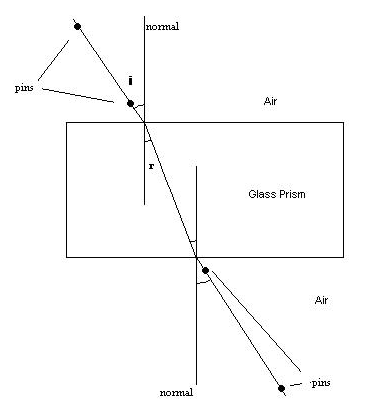
\includegraphics[width=10cm]{./img/rectangular-prism-1.png}
%\end{center}


\subsection{Measuring Refractive Index of Glass}

\subsubsection*{Learning Objectives}
\begin{itemize}
\item{To explain the refraction of a light ray from one medium to another} 
\item{To show the refraction of a ray of light at different angles} 
\item{To apply Snell's Law to find the refractive index of a medium by measuring incident and refracted angles} 
\item{To see the effect of refraction on an image} 
\end{itemize}

\subsubsection*{Background Information}
Light bends as it moves from one medium to another. When moving from a medium of low density to one of high density, a ray of light will bend inward towards the normal; when moving out again from the medium of high density to the medium of low density, the light ray will bend outward away from the normal.

Refracted light obeys Snell's Law, which states that $\ce{n1} \times \sin i = \ce{n2} \times \sin r$ where \ce{n1} is the refractive index of the first medium, $i$ is the incident angle of the light, \ce{n2} is the refractive index of the second medium and $r$ is the refracted angle of the light in the second medium. Because we know the refractive index of air, and we can measure the angles of incidence and refraction with a protractor, we can calculate the refractive index of any material.  

\subsubsection*{Materials}
Protractor from a mathematical set, pen, 30~cm square piece of thick cardboard from a box, piece of white paper, four-figure or calculator, tape or glue, 4 pins or syringe needles, rectangular glass block at least 6~mm thick from a glass shop (the glass block does not need to be large: 8~cm $\times$ 10~cm is easily enough). Often the glass block can be found for free, just make sure that the edges are even and that you can see through the block by looking through the edges.  

\subsubsection*{Hazards and Safety}
\begin{itemize}
\item{Be careful when using the glass.  If you are using a local glass block from a glass cutter, the edges may be sharp enough to cut skin.}
\item{If using syringe needles, use pliers or a hammer to bend the end of the needles so that they may not be used for any other purpose.}
\end{itemize}

\subsubsection*{Preparation Procedure}
\begin{enumerate}
\item{Collect all of the materials on a table.} 
\item{Tape or glue the white paper to the cardboard and cut the paper so that it is the same size as the cardboard.} 
\end{enumerate}

\subsubsection*{Activity Procedure}
\begin{enumerate}
\item{Place the cardboard flat on the table with the paper-side up.} 
\item{Place the glass block in the center of the paper and trace it with a pen.} 
\item{Remove the block from the paper; you should see its outline clearly from the pen.} 
\item{Use a protractor to draw a line perpendicular (90$^{\circ}$) near the center of one of the long sides of the glass block outline.} 
\item{Extend this line through both sides of the glass block so that on the paper you should have a picture of a rectangle with a line through its center.} 
\item{Where the line intersects one of the long sides of the rectangle, make a mark and label it $O$.}
\item{From the point $O$, draw a line outward at an angle of 10 degrees to the normal. Use a protractor to do this.} 
\item{Repeat this step to draw lines at angles of 20$^{\circ}$, 30$^{\circ}$, 40$^{\circ}$ and 50$^{\circ}$ to the normal, all converging on the point $O$.} 
\item{Replace the glass block in its outline on the paper.} 
\item{Place two pins or needles on the line for the incident light at 10$^{\circ}$. Place one of the pins close to the glass block and the other as far away as possible on the 10 degree line. The pins should stick upright easily in the cardboard}
\item{From the opposite side of the glass block, look through the block so that you can see the two pins on the other side through the block (do not look over the block).} 
\item{Close one eye and move left or right until the two pins you see through the block are perfectly aligned so that they look like one pin.} 
\item{On this side of the glass block, place another pin close to the block so that all three pins are aligned.} 
\item{Repeat this step with a fourth pin closer to your eye.} 
\item{Make sure that, as you look through the glass block, all four pins are aligned perfectly.} 
\item{Remove the pins on this side of the block and mark their positions (the holes in the paper) with a pen.} 
\item{Use the straight edge of the protractor to trace a line through the two points to the edge of the glass block.} 
\item{Mark this line as 10 degrees.} 
\item{Repeat steps 10 through 18 for the incident rays of 20, 30, 40 and 50 degrees. At the end you should have five lines coming from your side of the glass block at different points, each labeled with a different angle. These lines should be diverging from one another.} 
\item{Remove the glass block from the paper.} 
\item{Using the straight edge of the protractor, trace a line from $O$ to the point on the edge where the ray labeled ``10 degrees'' emerges.} 
\item{Repeat this step for each line so that you have five lines inside the glass block outline, each connecting point $O$ with one of the lines emerging from the block. These lines inside the block are the refracted rays corresponding to each of the incident rays (10, 20, 30, 40 and 50 degrees).} 
\item{Use the protractor to measure the angle between the normal inside the block and the first refracted ray.} 
\item{On a separate piece of paper, record the incident angle (10$^{\circ}$) and the corresponding refracted angle (which should be around 7$^{\circ}$, though this will change depending on the material you are using).} 
\item{Repeat these steps for the incident angles of 20, 30, 40 and 50 degrees and their respective refracted angles.} 
\item{Record these results in a table showing each incident angle and its respective refracted angle.} 
\item{Use a four-figure or calculator to find the Sine of each of these angles and record these in your table as well.} 
\item{Use a ruler to make a graph of $\sin r$ against $\sin i$. The x-axis (horizontal axis) should contain the values for the Sine of the incident angles, and the y-axis (vertical axis) should contain the values for the Sine of the refracted angles.} 
\item{Mark each of the five data points on the graph using your table of values for $\sin i$ and $\sin r$.} 
\item{Use a ruler or other straight edge to draw a straight line through the five points. Extend this line back through the y-axis (the axis containing values of $\sin r$).} 
\item{Calculate the slope of this line by using:%
$$\mathrm{slope} = \frac{\mathrm{change \;in \;}y}{\mathrm{change \;in \;}x}$$}
\item{Calculate the refractive index of glass by using:%
$$\mathrm{refractive \;index} = \frac{1}{\mathrm{slope}}$$} 
\end{enumerate}

\subsubsection*{Results and Conclusions}
It will be observed that the angle of a ray of light changes when moving from one medium to another.  An object seen through two or more media appears to be in a different place than where it actually is.  We can measure the angles of incidence and refraction, then use Snell's Law to find refractive index. 

\subsubsection*{Clean Up Procedure}
Return all supplies to their proper places making sure that the glass block is in a safe place where it will not break.

\subsubsection*{Discussion Questions}
\begin{enumerate}
\item{Why does light bend when moving from one medium to another?}
\item{In what direction does light bend when moving from a low-density medium to a high-density medium?}
\item{In what direction does light bend when moving from a high-density medium to a low-density medium?}
\item{What other materials could you use to measure refractive index instead of the glass block?}
\item{Why is it better to repeat the experiment for many angles of incidence instead of just one angle?}
\item{On the graph, what is the y-intercept? Why?}
\end{enumerate}

\subsubsection*{Notes}
This activity is very simple to perform but requires some practice, especially when trying to align all of the pins. Make sure that you can do the entire activity easily before you do it with students.  
Any material may be used; the glass block is only one option. Stained glass, water and plastic also work well.  
This activity appears often as a practical on the exams, so you can repeat it many times with students so that they know it very well.  



	%Real vs. Apparent Depth

	%Critical Angle / Total Internal Reflection
	
%\subsection{Pouring light}
%\begin{itemize}
%\item{Preparation Time: 5 minutes}
%\item{Materials: Opaque container (Nido can), nail, flashlight, regular container, water}
%\item{Procedure: Use the nail to poke a hole at the bottom of one side of the opaque container. Fill the container with water and allow the water to pour out into the other container. In a dark place, shine the flashlight down through the top of the opaque container: you will see the water glow as it is poured out.}
%\item{Theory: The light is reflected at the surface of water (total internal reflection), so when it travels through the stream of pouring water, it continues to be reflected inside the stream until it reaches the container below. The light that does escape the pouring water is what we see as the glowing effect.}
%\end{itemize}


\subsection{Total Internal Reflection in Water}

\subsubsection*{Learning Objectives}
\begin{itemize}
\item{To observe the effect of Total Internal Reflection of light inside water}
\end{itemize}

\subsubsection*{Background Information}
When light passes from a high-density medium to a low-density medium, it can undergo total internal reflection if the angle of incidence is great enough.  If light is passing through water, some of it will pass into air but some will be reflected at the surface back into the water.  This is the mechanism behind fibre-optic cables, which use total internal reflection in a clear wire to move light over great distances..

\subsubsection*{Materials}
Opaque container like a Nido can, nail, torch, water, bucket

\subsubsection*{Preparation Procedure}
\begin{enumerate}
\item{Use the nail to poke a hole at the bottom of one side of the opaque container.}
\end{enumerate}

\subsubsection*{Activity Procedure}
\begin{enumerate}
\item{Pour water into the opaque container so that it can flow out of the hole near the bottom into the other container.}
\item{In a dark room, shine a torch down into the water.}
\item{Observe the light in the water falling from the hole.}
\end{enumerate}

\subsubsection*{Results and Conclusions}
The light is reflected at the surface of water (total internal refection), so when it travels through the stream of pouring water, it continues to be reflected inside the stream until it reaches the container below. The light that only escapes farther down in the pouring water is what we see as the glowing
effect.

\subsubsection*{Cleanup Procedure}
Clean up the water and return materials to their proper places.

\subsubsection*{Discussion Questions}
\begin{enumerate}
\item{What causes the water to glow?}
\item{What is the light doing inside the water stream?}
\end{enumerate}

\subsubsection*{Notes}
While the light is being reflected inside the water stream, what we are seeing with our eyes is the light that escapes.  A certain percentage of light will escape each time it hits the surface of the water and air.  Light that enters the air at a small angle will escape and reach our eyes; light that hits at a large angle will be reflected again inside the water.


		%Periscope, Telescope, Binoculars
		
		
%Refraction by Lenses

\subsection{Focusing an Image through a Convex Lens}
\begin{itemize}
\item{Preparation Time: 1 minute}
\item{Materials: convex lens (magnifying glass on a Swiss army knife works well), white paper or screen, tissue paper (the paper used to wrap the Rexa toilet paper is perfect), pen, point light source (your headlamp, desk lamp, etc.), optional retort stands}
\item{Procedure: cut a piece of tissue paper to fit over your light source. Flatten this paper in a book overnight if necessary. Draw a thick arrow on this tissue paper and tape it over your light source. With students, set up the light source to shine directly on a white screen or paper about half a meter away. The distance depends on how strong the light is). Move the magnifying glass/convex lens back and forth between the light and screen until the image of the arrow is focused on the screen. Measure the distances from the lens to the screen and lens to the light source. Now you can calculate the focal length of the lens.}
\item{Variation: Fry some bugs with sunlight! If the sun is strong enough, you should be able to get paper to smoke, and no one likes siafu anyway.}
\item{Theory: The lens equation is given as 1/f = 1/u + 1/v where f is the focal length of the lens, u is the distance from the object to the lens, and v is the distance from the focused image to the lens. In our case, the object is out light source and arrow, and the image is on the white screen. By focusing the image, we set u and v, allowing us to calculate f.}
\end{itemize}


%Refraction through Prisms

\subsection{Refraction of Light Through Water}
\begin{itemize}
\item{Preparation Time: 5 minutes}
\item{Materials: cardstock or cardboard, jar, water, Nido or powdered soap, light source}
\item{Procedure: Cut a small hole, about half a cm, in the cardstock. Put some Nido or soap into the water in the jar so that it becomes cloudy. Shine the light through the hole in the card so that a thin beam can be seen in the cloudy water on the other side. Change the direction of the beam through the water to see the different refracted angles.}
\item{Theory: The Nido or soap provides particles in the water that will reflect light, clearly showing the path of the light through the water (picture headlights on a foggy day). Light slows down as it enters a denser medium, like water, from a less dense medium, like air. As such, the direction of the light changes in order to reduce the traveling time through the medium. This effect, called refraction, can be seen in the cloudy water.}
\end{itemize}


%Dispersion of White Light

%\subsection{Color wheel}
%\begin{itemize}
%\item{Preparation time: Half hour}
%\item{Materials: white paper, colored pencils, Nido can lid, 1” screw, tape or glue@Construction: Cut the paper into a circle with the same diameter as the Nido cap. Using a pencil and straight-edge, divide the circle into seven pie slices and color each slice a single color from ROYGBIV (Red, orange, yellow, green, blue, indigo, violet). Drawing 14 or 21 slices is more effective, but seven works well.@Using a pencil or something else sharp, balance the Nido lid until you find its center of gravity. Mark it and carefully screw the screw through at that point, creating a kind of top. Tape or glue the colored paper to the top, colored side up, screw point down. Now you have a top with the seven rainbow colors on top.}
%\item{Procedure: Review the colors with your students using the colors on the wheel/top/thing. Place the wheel on a desk and give it a good spin. If it is well-balanced, it should spin smoothly and all the colors run together to form white. Bask }
%\item{Variation: (1) Wrap string around the screw so that both ends of the string stick out. Pull them quickly in opposite directions to get the top spinning quickly. (2) Poke two holes about 1 cm on either side of the center of the wheel (no screw). Loop a string through the two holes so that two lengths of string of equal length stick out on each side. Tie the loose ends on the one side and then hook your thumbs into each loop. Twist the strings by spinning the wheel. If you pull, the wheel will spin and re-twist itself in the other direction. This is a child’s toy in many villages, so get one of your students to help you.}
%\item{Theory: For light, white is the presence of all colors (this is opposite for pigment). Theoretically, you could do this demo using only the three primary colors, but it might be harder to get the top to spin fast enough to lose all resolution of the colors. By using the seven rainbow colors, we make it easier for them to blend together; creating white as far as the eye is concerned.}
%\end{itemize}


\subsection{Newton Colour Wheel}

\subsubsection*{Learning Objectives}
\begin{itemize}
\item{To identify the colours of visible light in the electromagnetic spectrum} 
\item{To observe the mixing of colours to form white light} 
\end{itemize}

\subsubsection*{Background Information}
The colours of light are somehow different from the colours of pigment. The primary colours are red, green and blue, and the secondary colours are cyan, magenta and yellow. These are different from pigment. Also, when the colours of light are mixed, the product is white. White is the presence of all colours while black is the absence of all colours.  
By mixing the colours of light, we can see that they form white. The easiest way to mix colours is to use the spectrum of visible light, namely ROYGBIV, or Red, Orange, Yellow, Green, Blue, Indigo and Violet.  

\subsubsection*{Materials}
coloured pencils in red, orange, yellow, green, blue, indigo and violet; white paper, scissors, plastic lid to a Nido can or other container; 1-inch screw, tape or glue, optional compass from a mathematical set

\subsubsection*{Preparation Procedure}
\begin{enumerate}
\item{Place the plastic lid flat on the white paper.} 
\item{Use a pencil to trace the outline of the lid on the paper.} 
\item{Cut the circle of paper out.} 
\item{Use a pencil to divide the circle into seven equal slices meeting at the center of the circle.  If you have a compass it can be used to divide the circle more evenly into seven slices.} 
\item{Find the center of mass of the plastic lid by balancing it on a pencil.} 
\item{Thread the screw through the center of the lid so that it sticks out the bottom of the lid and is flat on top.} 
\item{Tape or glue the coloured paper to the top of the lid.} 
\end{enumerate}

\subsubsection*{Activity Procedure}
\begin{enumerate}
\item{Hold the colour wheel on a table so that the wheel balances on the tip of the screw and the colours face upward.} 
\item{Spin the wheel between your fingers so that it spins on its own on the table.} 
\item{Observe the change in colour.} 
\end{enumerate}

\subsubsection*{Results and Conclusions}
When the colour wheel is stationary, all seven colours can be seen clearly. When the wheel spins quickly, the colours blend together to form white. This is because when all the colours of light are mixed, white is produced.  

\subsubsection*{Clean Up Procedure}
Return all materials to their proper places.

\subsubsection*{Discussion Questions}
\begin{enumerate}
\item{What are the colours on the colour wheel?}
\item{Why is it better to use all the colours rather than just a few?}
\item{What colour is seen on the wheel when it is spinning quickly.} 
\end{enumerate}

\subsubsection*{Notes}
The colour wheel works best if the screw is placed in the exact center of the plastic lid. If it is off center, the wheel will not spin well. Also, you can get a clearer white colour if you divide the wheel into more sections of colour. 14 is better than 7, though 7 will work well.  


\subsection{Dispersion of White Light: Part 1}

\subsubsection*{Learning Objectives}
\begin{itemize}
\item{To demonstrate the dispersion of white light} 
\end{itemize}

\subsubsection*{Background Information}
White light is light which contains all colours.  The light from the sun and some bulbs is white light, so we can divide it into its component colours.  When light travels from air to a denser material, each wavelength of light (colour) bends at a different angle so the white light splits into all the colours of the visible spectrum, of which the most visible are red, orange, yellow, green, blue, indigo and violet (ROYGBIV). This may be easily shown by placing a mirror in a basin of water, as shown below:


% WRONG PIC!!
%\begin{figure}
%\begin{center}
%\def\svgwidth{150pt}
%\input{./img/dispersion-white-light.pdf_tex}
%\caption{Dispersion of White Light by a Mirror in Water}
%\label{fig:dispersion-white-light}
%\end{center}
%\end{figure}

The dispersion of light may also be shown with soap bubbles, as discussed in the followin activity.

\subsubsection*{Materials}
Water, soap, beaker*, light, and straw

\subsubsection*{Preparation Procedure}
Make a soap solution by mixing water and soap.

\subsubsection*{Activity Procedure}
\begin{enumerate}
\item{Place the beaker with the soap solution near a source of white light or in open sunlight.} 
\item{Immerse the straw into the soap solution and blow into it to form bubbles.} 
\item{Describe and record any observations.} 
\end{enumerate}

\subsubsection*{Results and Conclusions}
Different colours are observed as the sunlight hits the soapy bubbles and undergoes refraction into its component colours.  This is because the light is refracted when passing into the soap and then again when passing back into air.

\subsubsection*{Clean Up Procedure}
Collect all materials and return them to their proper place.

\subsubsection*{Discussion Question}
What colours did you see in the soap bubbles? Why?

\subsubsection*{Notes}
The dividing of white light into its colours is called dispersion.  Dispersion of sunlight can be observed in a rainbow, a thin layer or oil or soap, etc.  This can be demonstrated most easily with soap bubbles or a triangular prism.

	% Dispersion of White Light: Part 2 ???
	% Use pic from Part 1


\subsection{Thin Film Interference}
\begin{itemize}
\item{Preparation time: 5 minutes}
\item{Materials: A small bowl or other dish, water, oil}
\item{Procedure: Pour water into the dish. Touch your finger to the oil, then to the surface of the water. A small amount of oil should be transferred to the surface of the water, where it will form a thin film. A colorful rainbow pattern should be visible in the thin film. Try looking at it from different angles. If you are having trouble seeing the colors try moving the dish into brighter light (direct sunlight works well), or using a dark-colored dish.}
\item{Theory: When light strikes the surface of the water, some is reflected off the top of the film of oil, and some is reflected from the oil-water interface. When the difference in the path length between these two paths is an integer number of wavelengths, light of that wavelength will be strongly seen. This gives rise to the rainbow pattern.}
\end{itemize}

\subsection{Water Prism}
\begin{itemize}
\item{Preparation Time: 1 minute}
\item{Materials: mirror, clear rectangular container, water, white light source}
\item{Procedure: Fill the container with water. On the inside of one of the sides, place the mirror with the reflective side facing in. In a dark place, shine a light through the opposite side of the container at an angle so that the light passes through the water, reflects off the mirror, and exits the container on the original side. The light leaving the container should be dispersed into the color spectrum.}
\item{Theory: Light refracts when entering a dense medium like water. As white light is refracted, each color that makes up the white light (the whole color spectrum) refracts at a different angle depending on its wavelength, and so a refracted ray creates a slight rainbow pattern. Normally this effect can be seen only partially as white light passes through water, but as you are refracting the water twice, once into the water and once back into air, the dispersion effect will have twice the magnitude.}
\end{itemize}

%Colour

